% Figure 2: full-model correctness, read against the platform's own noise floor.
%
% Build: tectonic docs/figures/fig2_correctness.tex
%
% Measured on 8x H100 SXM5, TP8, the real 975B NVFP4 checkpoint.
% Source: journal/remote/gate_logit_parity_8xh100.json
%   parity.mean                  0.0477  (ours vs stock)
%   batch_consistency.stock.mean 0.1496  (stock vs stock, batched vs single)
%   batch_consistency.ours.mean  0.1628  (ours vs ours,   batched vs single)
%   parity.tokens_match_all      true, 32/32 prompts, 2369 tokens
%
% The two grey bars are the same build disagreeing with itself. They are the
% floor any cross-build comparison must be read against. Bars are valid here
% because the axis is linear.
%
% Note on tikz: put text= after fill=, never color=. color= overwrites draw
% and fill, which silently turned this figure's callout box black once.

\documentclass[border=14pt]{standalone}
% Shared style for all Inkling-turbo figures.
% Included by each standalone figure so they read as one family.
\usepackage{tikz}
\usepackage{pgfplots}
\pgfplotsset{compat=1.18}
\usetikzlibrary{calc,plotmarks,backgrounds}

% palette
\definecolor{ours}{HTML}{0B6E6A}     % our kernel
\definecolor{floorc}{HTML}{64748B}   % the biasless floor
\definecolor{prod}{HTML}{C2410C}     % the path vLLM ships
\definecolor{altA}{HTML}{9A3412}     % other day-0 paths
\definecolor{altB}{HTML}{78350F}
\definecolor{ink}{HTML}{111827}      % text
\definecolor{guide}{HTML}{DDE1E6}    % grid
\definecolor{band}{HTML}{F4F6F8}     % group banding
\definecolor{okc}{HTML}{15803D}      % validated
\definecolor{partc}{HTML}{B45309}    % partial

% shared axis look: no frame, no ticks, faint grid, small labels
\pgfplotsset{
  inkling/.style={
    scale only axis,
    axis line style={draw=none},
    tick style={draw=none},
    grid style={line width=0.45pt, color=guide},
    xticklabel style={font=\scriptsize, color=ink!62},
    yticklabel style={font=\scriptsize, color=ink!88},
    xlabel style={font=\footnotesize, color=ink!85},
    ylabel style={font=\footnotesize, color=ink!85},
    clip=false,
  },
}

% figure title + standfirst, placed above a named axis
\newcommand{\figtitle}[3]{%
  % #1 axis name, #2 title, #3 standfirst
  \node[anchor=north west, font=\bfseries, color=ink]
    at ($(#1.north west)+(\titleoffset,\titletop)$) {\large #2};
  \node[anchor=north west, font=\scriptsize, color=ink!58,
        text width=\standfirstwidth]
    at ($(#1.north west)+(\titleoffset,\titlesub)$) {#3};
}


\def\titleoffset{-6.15cm}
\def\titletop{1.72cm}
\def\titlesub{1.28cm}
\def\standfirstwidth{16.4cm}

\begin{document}
\sffamily
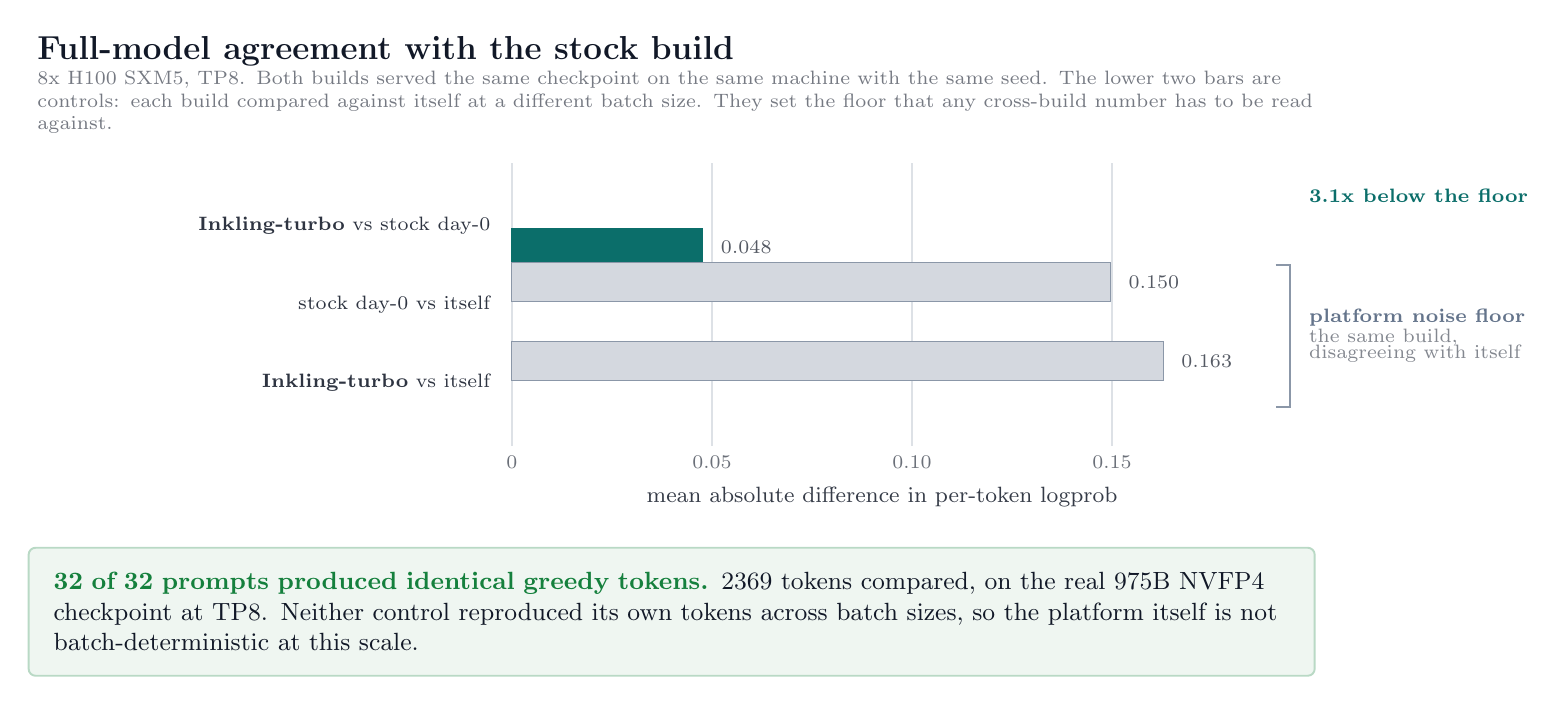
\begin{tikzpicture}[font=\sffamily]

\begin{axis}[
  inkling,
  name=A,
  width=9.4cm, height=3.6cm,
  xbar,
  bar width=14pt,
  xmin=0, xmax=0.185,
  xtick={0,0.05,0.10,0.15},
  xticklabels={0,0.05,0.10,0.15},
  xlabel={mean absolute difference in per-token logprob},
  ymin=-0.8, ymax=2.8,
  ytick={0,1,2},
  yticklabels={
    {\textbf{Inkling-turbo} vs itself},
    {stock day-0 vs itself},
    {\textbf{Inkling-turbo} vs stock day-0}},
  xmajorgrids,
  nodes near coords,
  nodes near coords style={font=\scriptsize, color=ink!72, anchor=west,
                           xshift=3pt, /pgf/number format/fixed,
                           /pgf/number format/precision=3,
                           /pgf/number format/fixed zerofill},
]

\addplot[fill=ours, draw=ours] coordinates {(0.0477,2)};
\addplot[fill=floorc!28, draw=floorc!75] coordinates {(0.1496,1) (0.1628,0)};

\end{axis}

% ---- bracket marking the two controls as the noise floor
\draw[floorc!75, line width=0.8pt]
  ($(A.north east)+(0.30cm,-1.30cm)$) --
  ($(A.north east)+(0.48cm,-1.30cm)$) --
  ($(A.north east)+(0.48cm,-3.10cm)$) --
  ($(A.north east)+(0.30cm,-3.10cm)$);
\node[anchor=west, font=\scriptsize, color=floorc, align=left]
  at ($(A.north east)+(0.60cm,-2.20cm)$)
  {\textbf{platform noise floor}\\[-1pt]
   {\color{ink!52}the same build,}\\[-2pt]
   {\color{ink!52}disagreeing with itself}};

\node[anchor=west, font=\scriptsize\bfseries, color=ours]
  at ($(A.north east)+(0.60cm,-0.42cm)$) {3.1x below the floor};

% ---- headline result. text= after fill=, so the fill survives.
\node[anchor=north west, draw=okc!30, fill=okc!7, rounded corners=2.5pt,
      line width=0.7pt, inner sep=9pt, text width=15.7cm, align=left,
      font=\small, text=ink]
  at ($(A.south west)+(-6.15cm,-1.28cm)$)
  {\textbf{\color{okc}32 of 32 prompts produced identical greedy tokens.}
   2369 tokens compared, on the real 975B NVFP4 checkpoint at TP8. Neither
   control reproduced its own tokens across batch sizes, so the platform
   itself is not batch-deterministic at this scale.};

\figtitle{A}{Full-model agreement with the stock build}{%
  8x H100 SXM5, TP8. Both builds served the same checkpoint on the same
  machine with the same seed. The lower two bars are controls: each build
  compared against itself at a different batch size. They set the floor that
  any cross-build number has to be read against.}

\end{tikzpicture}
\end{document}
